\newcommand\resS   [0]{\Large28}
\newcommand\resSF  [0]{\Large3}
\newcommand\resSFA [0]{\Large16}
\newcommand\resSA  [0]{\Large77}
\newcommand\resF   [0]{\Large1}
\newcommand\resFA  [0]{\Large6}
\newcommand\resP   [0]{\Large37}
\newcommand\resPA  [0]{\Large37}
\newcommand\resA   [0]{\Large9}

\tikzset{
  every node/.style={scale=0.6}
}
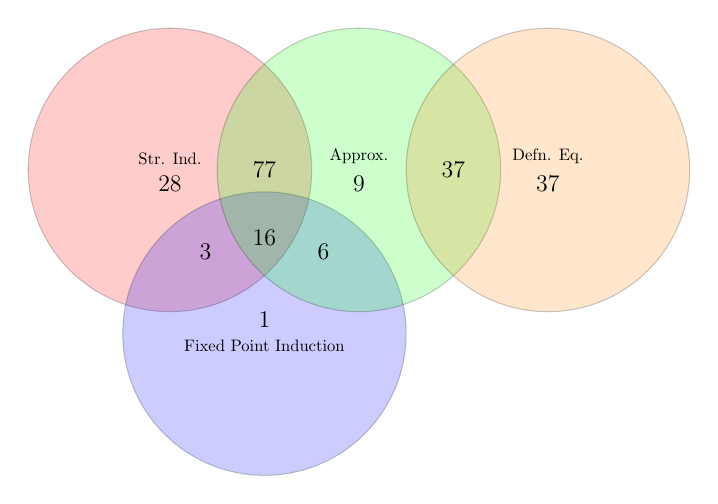
\begin{tikzpicture}[scale=0.6]
  \tikzset{venn circle/.style={draw,circle,minimum width=6cm,fill=#1,opacity=0.2}}

  \node [venn circle = red]    (S) at (0,0)                              {};
  \node [venn circle = blue]   (F) at (-60:4cm)                          {};
  \node [venn circle = green]  (A) at (0:4cm)                            {};
  \node [venn circle = orange] (P) at (0:8cm)                            {};
  \node [above]                    at (barycentric cs:S=1)               {Str. Ind.};
  \node [below]                    at (barycentric cs:S=1)               {\resS};
  \node [above]                    at (barycentric cs:F=1)               {\resF};
  \node [below]                    at (barycentric cs:F=1)               {Fixed Point Induction};
  \node [above]                    at (barycentric cs:A=1)               {Approx.};
  \node [below]                    at (barycentric cs:A=1)               {\resA};
  \node [above]                    at (barycentric cs:P=1)               {Defn. Eq.};
  \node [below]                    at (barycentric cs:P=1)               {\resP};
  \node [left]                     at (barycentric cs:S=1/2,F=1/2)       {\resSF};
  \node                            at (barycentric cs:S=1/2,A=1/2)       {\resSA};
  \node [right]                    at (barycentric cs:F=1/2,A=1/2)       {\resFA};
  \node [below]                    at (barycentric cs:S=1/3,F=1/3,A=1/3) {\resSFA};
  \node                            at (barycentric cs:A=1/2,P=1/2)       {\resPA};

\end{tikzpicture}
